% \chapter{Removing assumptions in joint dynamics system identification}
% \chapter{Removing assumptions using ultrafast ultrasound}

% ===========================================================================
\chapter{Relaxing assumptions in joint dynamics system identification using ultrafast ultrasound}
\label{chap:remove_assumptions}
% Chapter intro: discussion on how (some of) the assumptions can be removed by using ultrafast ultrasound. 
% Focus on IDing ankle joint dynamics, since earlier study showed that (Ossenkoppele) 
% “The flexor and extensor muscles of the wrist have a large ratio of tendon length to muscle fibre length and this ratio is even larger for the flexor and extensor muscles of the ankle [134, Zajac].”

In chapter 2, two modalities of ultrafast ultrasound that can be used in system identification were described, i.e. elastography and imaging. The previous chapter described the most important assumptions present in neuromuscular models, and discussed their implications.  This chapter will discuss in what way the two modalities of ultrafast ultrasound can be used to relax the assumptions in the current neuromuscular models.

The focus of this chapter will be on identification of ankle joint dynamics, since previous explorative work showed that the imaging of lower leg muscles and subsequent analysis of the ultrasound images is considered easier compared to e.g. the wrist joint, due to larger sized and fewer muscles in the lower leg \cite{ossenkoppele_ultrasound_2017}. Furthermore, due to the relatively large tendon slack length, as defined by \citeauthor{zajac_muscle_1989} as the ratio between tendon rest length and optimal muscle fibre length \cite{zajac_muscle_1989}, in the lower leg extensor and flexor muscles, interesting muscle tendon interaction can be expected. 



% ===========================================================================
% MOVED TO CHAPTER 3
%\section{Implication of assumptions}
% NOTE: all assumptions are closelty interconnected, hence a clear separation is hard to do. Two main assumptions to which the others are closely related will be discussed, and the implications thereof. 
%There is a wide variety in modelling of the neuromuscular system across the studies, based on various assumptions. The wide variety in modelling approaches shows that not all studies have the same goal. Where \cite{kearney_identification_1997, mirbagheri_intrinsic_2000, de_gooijer-van_de_groep_estimation_2016, jalaleddini_subspace_2017} used a model with as little as possible \textit{a priori} knowledge, other studies attempted to build (simplified) models based on the current believes about the human physiology involved with reflexes and movement \cite{zhang_simultaneous_1997, van_der_helm_identification_2002, schouten_nmclab_2008, mugge_rigorous_2010}. The former can be seen as more phenomenological studies, which can be used to determine characteristic differences between populations, but are not as informative as the latter, where the goal is to improve the understanding of the underlying physiology and relate changes in the physiologic state to the observed behaviour. Hence, the various identified assumptions all lead to some implications for system identification of the joint dynamics, and have a great influence on what exactly can be learned from the experiment and model. Since the assumptions and their implications are for the most part closely related, these cannot be clearly separated. Therefore, the implications will be discussed based on two main assumptions, relating to muscle-tendon interaction and lumping of muscles. 
%
%
%\subsection{Muscle-tendon interaction}
%A number of system identification studies did not consider muscle-tendon interaction, and consequently related joint ankle or position directly to muscle elongation \cite{zhang_simultaneous_1997, kearney_identification_1997, mirbagheri_intrinsic_2000, van_der_helm_identification_2002, de_gooijer-van_de_groep_estimation_2016}. When it is assumed that no MTU interaction occurs, this directly implies an infinitely stiff tendon. Especially for compliant tendons, such as the Achilles tendon connected to the plantar flexors in the lower leg, significant MTU interaction can be expected, which can lead to a distorted estimation of the muscle elongation. This has consequences for the separation of intrinsic and reflexive contributions to the movement. 
%
%Not considering MTU interaction can lead to a distorted estimation of muscle elongation and subsequently distortion in the estimated contribution of intrinsic properties to movement. In general, a simple spring-damper system consisting of two parameters is used to describe the intrinsic properties of all muscles, passive tissue, tendons and joint resistance. Since these components do not all displace the same amount due to MTU interaction and different moment arms, the estimation of intrinsic properties is distorted (further discussed in \autoref{sec:rem_lumping-muscle}). 
%
%Likewise, the distorted estimation of muscle elongation has implications on the degree of proprioceptive afferent activity leading to modulation of reflexes. The muscle spindles are sensitive to muscle elongation and lengthening velocity, which in case of an infinitely stiff tendon would be overestimated, since all the elongation is ascribed to the muscle. Some studies considered either position or velocity feedback, which has proven to result in models with reasonable \textit{variance accounted for} (VAF), but presumably leads to further overestimation of a single component to reflex modulation \cite{maas_is_2009}. Furthermore, all of the studies that did not model muscle-tendon interaction also omitted the Golgi tendon organ (i.e. force) afferent feedback. Omission of force feedback can further lead to overestimation of the modelled reflexive mechanism. The choice of proprioceptive receptor modelling does not seem to have a large influence on the prediction capabilities of the model (in terms of VAF), but do not necessarily resemble the physiology behind reflex modulation. 
%% point about tendon in series, stiffness lot higher than muscle in passive state, hence due to 1/keq = 1/k1 + 1/k2 minor contribution. However, for fast movements, this is not the case.
%
%Especially the omission of GTO force feedback contradicts findings reported by the group of Sinkjaer. Af Klint et al. found strong support for contribution of GTO feedback in addition to MS feedback in adaptations to ground irregularities during locomotion \cite{klint_afferent_2009}. However, the effect of GTO and MS feedback during locomotion appeared to be stance phase dependent, where respectively mid-stance MS feedback and late-stance GTO feedback was thought to be dominant \cite{grey_positive_2007, af_klint_sudden_2009}. This emphasises the need for additional measurement data, enabling further isolation of afferent activity during other motor tasks (i.e. balance, force, position tasks). 
%
%	% \tred[expected GTO feedback? Sinkjaer, af Klint??] \textcolor{red}{\lipsum[1]}
%	% - when not considered, GTO omitted. no physiological basis refl modulation
%	%     - expected role is substantial (sinkjaer, klint... ??)
%	% - Wrong estimation leads to wrong activation signal when considering afferent feedback
%
%
%\subsection{Lumping muscle structure}
%\label{sec:rem_lumping-muscle}
%A very common simplification of the neuromuscular model is lumping of antagonistic muscle groups \cite{zhang_simultaneous_1997, van_der_helm_identification_2002, schouten_nmclab_2008, mugge_rigorous_2010}. This has as advantage that the model can be defined by less parameters compared to an antagonistic model (e.g. \cite{de_gooijer-van_de_groep_estimation_2016}). No moment arms for MTUs have to be estimated or averaged over multiple MTUs for the same function (i.e. flexion versus extension). Furthermore, the intrinsic properties (i.e. inertia, stiffness and damping) of limb, joint resistance, tendon, passive and active muscle tissue can all be lumped into a minimum of three parameters. The lumping of muscle groups with different function does however also have disadvantages when the intrinsic and reflexive effects on movements are under analysis. 
%
%% - afferent inhibity/excit contribution. Goal is to separate how the reflexive contribition is build up. with this lumping, Ia, Ib and II afferents of muscle groups contribution to modulation cannot be determined. physiology behind this remains elusive. 
%Firstly, due to lumping the afferent GTO and MS feedback from muscle groups with different functions cannot be well separated. \tred[However, the different muscle groups are always making opposite movements, so the afferent signals are expected to be opposite.] To get a better understanding of reflex modulation, a separation of the afferent signals form the different groups is required, which means that the flexors and extensors have to be lumped separately. In simulation studies (e.g. \cite{mugge_modeling_2012}) this separation is relatively straightforward, but the large number of additional parameters make this approach impractical for identification studies. Although the study of \citeauthor{de_gooijer-van_de_groep_estimation_2016} did use an antagonistic model \cite{de_gooijer-van_de_groep_estimation_2016}, fitting the model might only be possible under specific experimental conditions. This hampers the use of such an antagonistic model in system identification experiments were wide bandwidth perturbation signals are used (further discussed in \autoref{sec:rem_incompatibility}).
%
%% - nonlinear properties proprioceptors only under specific conditions. 
%Secondly, the nonlinear properties of the proprioceptors cannot accurately be modelled and identified with a fully lumped muscle model. The muscle spindles are only sensitive to muscle lengthening and Golgi tendon organs are mostly sensitive to active muscle force. For GTO force feedback a simple gain with a time delay is typically used \cite{schouten_nmclab_2008, mugge_rigorous_2010}. Apart from the nonlinearity of the GTO itself, the flexor and extensor muscles often have asymmetric force characteristics (e.g. plantar flexors stronger than dorsiflexors \cite{fukunaga_specific_1996}). Consequently, modelling the GTOs in plantar flexor and dorsiflexor muscles with a single linear gain could result in an overestimation of plantar flexor MTU force contribution to the afferent signal. The lumping in combination with no MTU interaction has as a consequence that the source of the afferent activity per muscle group \tred[can never be found]. 
%
%% - intrinsic estimated properties do not resemble underlying physoilogy, but contaminated. This does not imply that this is incorrect, but applying new tech UUS that provides specific quantitative data about specific (sub)module creates mismatch. 
%Lastly, the lumping of intrinsic parameters makes the system identification and parameter estimation easier, but does not result in parameters that have a direct physiological meaning. Furthermore, the parameters that are defined, possibly do not only contain contributions of the modelled structure, but are contaminated by contributions of other tissue, e.g. joint resistance. This is not wrong on its own, but has consequences for the usefulness of additional measurement data that has a direct physiological basis (e.g. viscoelastic properties of tendon and muscle). This incompatibility of data and current models will be further discussed in \autoref{sec:rem_incompatibility}. 
%
%% - separation of muscle groups is not that straightforward. apart from more parameters in current model doubled, muscle model, more parameters due to introduction of moment arms, more tendon, joint friction for example not as easily lumped. A view on what these implications mean for the neuromuscular model is presented in last section. 
%
%
%
%% \subsection{Overview implications and what ultrasound can mean}
%% Relate assumptions to goals? 
%% table goals, and which technology can fulfil them. 
%




% \newpage
% ===========================================================================
\section{Assessing intrinsic properties -- Shear wave elastography}
One possibility that ultrafast ultrasound offers is performing quantitative elastography on various tissue types. Two different methods, supersonic shear wave imaging (SSI, purely elastic, see \autoref{sec:us_ssi}) and shear wave spectroscopy (SWS, viscoelastic, see \ref{sec:us_sws}) have been used in various studies, to assess the mechanical properties of tendon and muscle under various conditions. This section will show some of these studies and discuss their methods and limitations. Finally, it will be discussed in what way elastography can be of value in system identification studies. 



\subsection{Muscle properties}
%There is some variation in the methods used to assess the mechanical properties of the muscle. 

% GENNISSON 1
\begin{figure}[t]
	\centering
	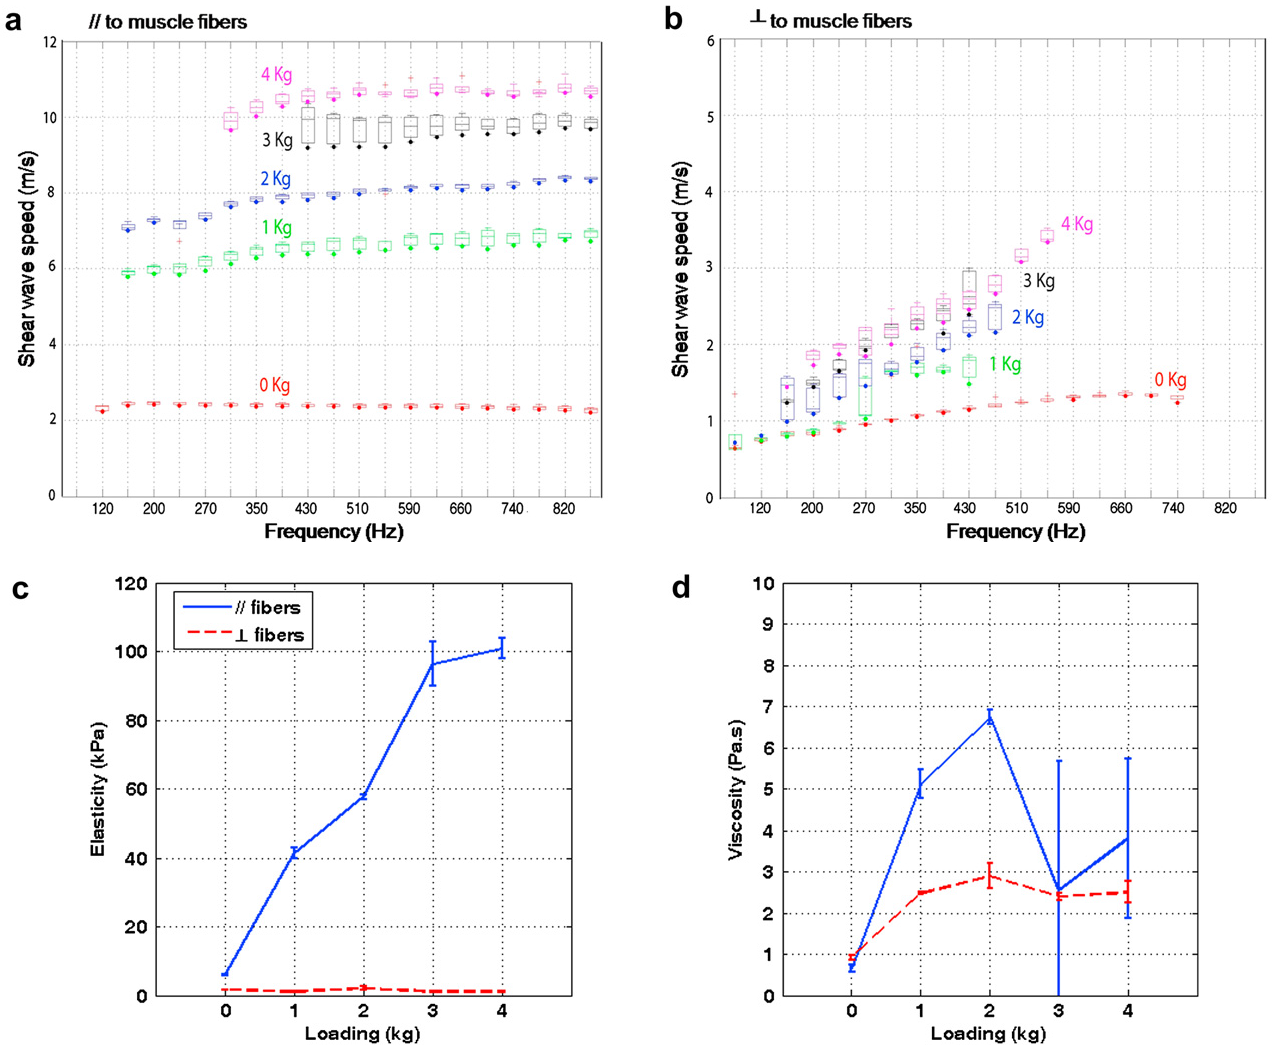
\includegraphics[width=.90\linewidth]{Figures/elastography/gennisson_dispersion2.png}
	\caption{Shear wave speed and estimated mechanical properties for the human \textit{brachialis} muscle under various loads, with elbow flexion of \SI{90}{\deg}. \textbf{(a,b)} Shear phase velocity over frequency under various loads for one subject, \textbf{(a)} parallel to muscle fibres and \textbf{(b)} perpendicular to muscle fibres. \textbf{(c,d)} Estimated mechanical properties using a Voigt model under increasing load, \textbf{(c)} shear elasticity and \textbf{(d)} shear viscosity. Figure adapted from \citet{gennisson_viscoelastic_2010}.}
	\label{fig:rem_gennisson_dispersion_force}
\end{figure}


\citeauthor{gennisson_viscoelastic_2010} used both SSI and SWS to assess the mechanical properties of the \textit{brachialis} muscle under various conditions \cite{gennisson_viscoelastic_2010}. The elastic properties were assessed parallel and perpendicular to the muscle fibres, with the elbow at \SI{90}{\deg} flexion under isometric contraction of the \textit{brachialis}, with loads increasing from 0 to \SI{5}{\kilogram} with increments of \SI{1}{\kilogram}. It was found that shear modulus $\mu$ increased with contraction level from 4.0 to \SI{36.6}{\kilo\pascal} along the fibres and from 2.3 to \SI{4.0}{\kilo\pascal} perpendicular to the fibres, highlighting the anisotropic properties of muscle tissue. SWS was also performed under the same load conditions as SSI. It was found that the shear wave phase velocity only increased slightly with frequency parallel to the muscle fibres (similar to findings \citet{deffieux_shear_2009}), but strongly perpendicular to the fibres (see \autoref{fig:rem_gennisson_dispersion_force}a,b). The muscle can thus be considered non-dispersive parallel to the fibres under these conditions (elbow flexion \SI{90}{\deg}). SSI was also performed to assess the passive properties of the muscle, by increasing the elbow angle from 90 to \SI{165}{\deg} with steps of \SI{25}{\deg}. It was found that the shear wave group velocity increased strongly from \SI{2.7}{\meter\per\second} to \SI{5.7}{\meter\per\second} along the fibres, and slowly from \SI{1.2}{\meter\per\second} to \SI{1.8}{\meter\per\second} perpendicular to the fibres (\autoref{fig:rem_gennisson_dispersion_passive}a). The viscoelastic parameters resulting from the dispersion analysis are depicted in \autoref{fig:rem_gennisson_dispersion_passive}b. %It can be seen that the shear elasticity increases strongly with elbow angle, which is in correspondence 


The SWS method has been used to compare the dispersion in stroke-paretic muscles to contralateral muscles during passive \cite{rasool_altered_2016} and active \cite{saadat_frequency_2018} conditions. In study of \citet{rasool_altered_2016}, the biceps muscle was fixed to an elbow flexion angle of \SI{120}{\deg} in a passive state (validated by EMG activity measurement), and SSI and SWS measurements were conducted. It was found that the group velocity was significantly higher in stroke-affected muscles, indicating increased stiffness. Furthermore, a difference in dispersion was found, the phase velocity was observed to be higher over all frequencies in stroke-affected muscles (not significant) \cite{rasool_altered_2016}. 

\citet{saadat_frequency_2018} measured the shear wave dispersion under both active and passive conditions (0\%, 10\%, 20\% and 30\% of MVC), with elbow flexion of \SI{150}{\deg}. It was found that the shear wave phase velocity was higher across all frequencies in the contralateral muscles with respect to the paretic muscles (see \autoref{fig:saadat_dispersion_paretic}). In the passive condition, the opposite was found, in correspondence with the findings of \citeauthor{rasool_altered_2016} \cite{saadat_frequency_2018}. In neither of these two studies a rheological model was fit to the dispersion curves, hence no mechanical parameters were estimated. 


%In 2011, Arda and collaborators (5) performed a study of SWE that included the gastrocnemius and masseter muscles and the supraspinatus and Achilles tendons, in 127 healthy volunteers of both sexes in both the longitudinal and transverse planes, to determine the normal measurement values of different healthy tissues. 



% GENNISSON 2
\begin{figure}[t]
	\centering
	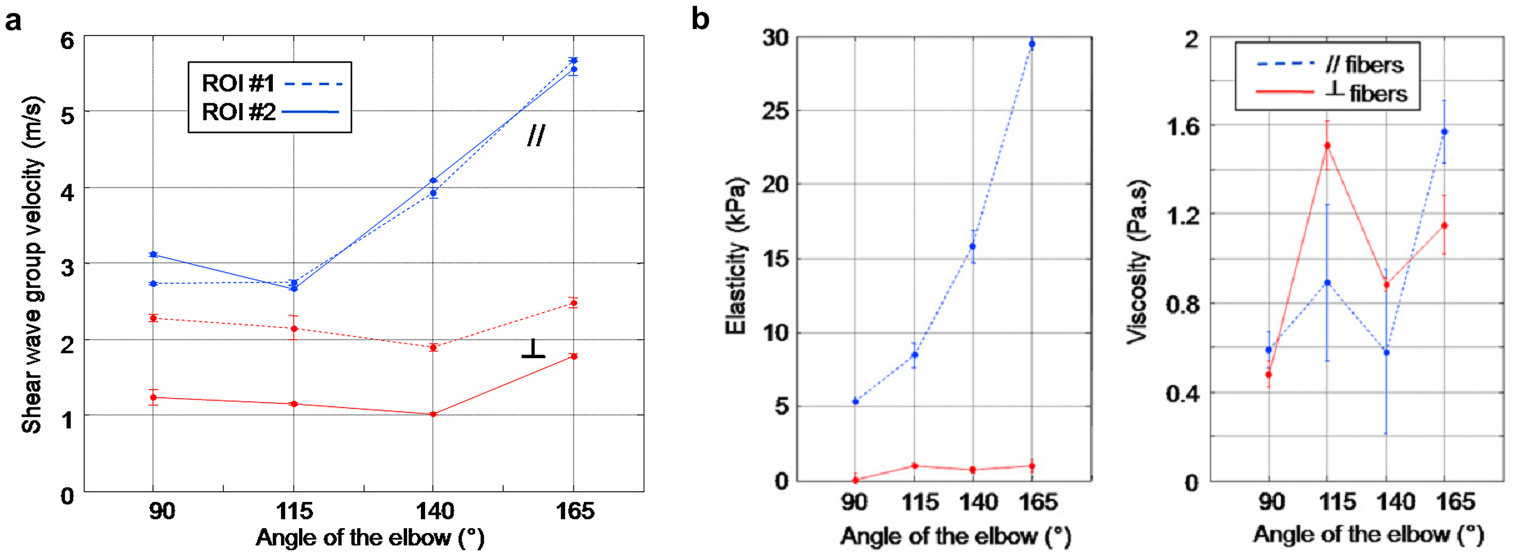
\includegraphics[width=.95\linewidth]{Figures/elastography/gennisson_dispersion_passive.png}
	\caption{\textbf{(a)} Shear group velocity in the  \textit{biceps brachii} (ROI 1) and \textit{brachialis} (ROI 2) along and perpendicular to the muscle fibers, for different levels of elbow extension. \textbf{(b)} Estimated viscoelastic parameters for the \textit{brachialis} muscle. Figure adapted from \citet{gennisson_viscoelastic_2010}.}
	\label{fig:rem_gennisson_dispersion_passive}
\end{figure}

% SAADET
\begin{figure}[t]
	\centering
	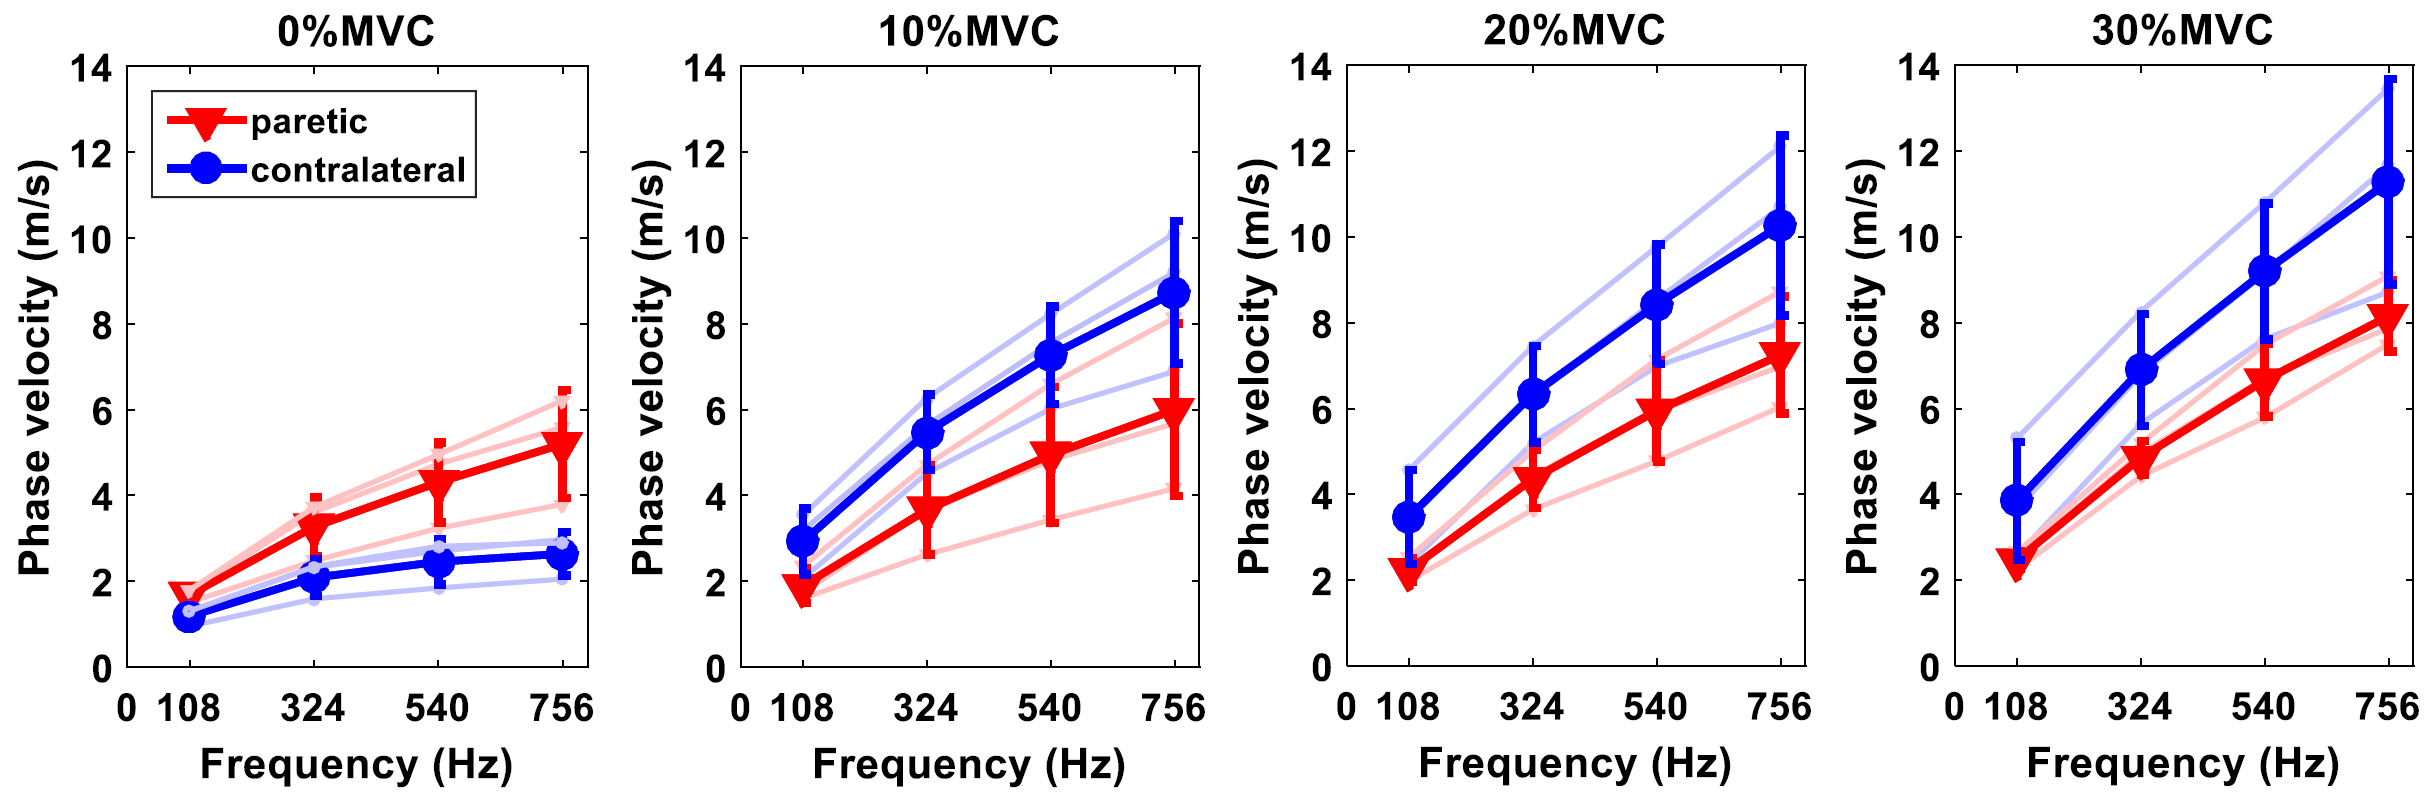
\includegraphics[width=.95\linewidth]{Figures/elastography/saadat_dispersion_paretic.png}
	\caption{Shear wave phase velocity in the biceps muscle over frequency (elbow flexion \SI{150}{\deg}), for multiple levels of contraction. It can be seen that in all the active conditions the phase velocity is lower over all frequencies for paretic muscles compared to the contralateral muscles. Figure adapted from \citet{saadat_frequency_2018}.}
	\label{fig:saadat_dispersion_paretic}
\end{figure}


\subsubsection{Conflicting reports on muscle dispersion}
In the studies by \citeauthor{deffieux_shear_2009} (\textit{biceps brachii}, experimental conditions not described) and \citeauthor{gennisson_viscoelastic_2010} (\textit{brachialis}, elbow \SI{90}{\deg} flexion) the muscle was found to be nondispersive parallel to the fibres (both studies from the group of Tanter and Fink) \cite{deffieux_shear_2009, gennisson_viscoelastic_2010}. By contrast, \citeauthor{rasool_altered_2016} and \citeauthor{saadat_frequency_2018} did found high dispersion when performing SWS parallel to the muscle fibres \cite{rasool_altered_2016, saadat_frequency_2018}. A later study by \citeauthor{rasool_shear_2018}, comparing stroke-affected to contralateral muscles, also reports high dispersion (\textit{biceps brachii}, passive condition, 90, 120 and 150 \si{\deg} elbow flexion) \cite{rasool_shear_2018}. Other than these studies, there are no more studies that performed a dispersion analysis on the SSI measurements from muscles. 

It is hard to find the source of this discrepancy in literature, possible sources are individual differences between participants, different experimental conditions or differences in data analysis. Regarding influence of analysis method, \citet{rasool_shear_2018} reported a great influence of local minima in the optimization procedure (Matlab \texttt{lsqnonlin}, least squares) for fitting the $\mu_1$ and $\mu_2$ parameters of the Voigt model to the measured dispersion curves. This does however not explain the discrepancy in the dispersion curves itself, as these follow directly from the tracked shear wave. %It can only explain differences in reported material parameters in past and future studies. 

%\tred[discussion parameter fit analysis?]


\subsubsection{Estimation of individual muscle force}
\citet{bouillard_estimation_2011} used SSI to estimate individual muscle force in the \textit{abductor digitimi minimi} and \textit{first dorsal interosseous} muscles, and validated the results by EMG to force conversion methods. These muscles were chosen because these are muscles without synergists for abduction. Consequently, the measured torque could be related to the measured EMG activation. Subjects were asked to perform isometric ramp contractions from 0\% to 30\% MVC for the \textit{abductor digitimi minimi} and 0\% to 60\% MVC for the \textit{first dorsal interosseous}, within \SI{30}{\second}. In a second trial, subjects had to randomly move their finger, while keeping the MVC between the same level as during the ramp contractions. EMG and SSI measurements were done on two separate days (separated by 45 hours). The SSI measurements were performed at \SI{1}{\hertz}, which was the maximum sample frequency of the SSI equipment (Aixplorer version 4.2, Supersonic Imagine, Aix en Provence, France). Two separate simple linear models were fitted to estimate the abduction torque from either shear elastic modulus or EMG. It was found that the model based on SSI measurements was significantly more accurate in predicting torque than the EMG model. 
A later study by \citet{ates_muscle_2015} also found a linear relation between shear elastic modulus (measured with SSI at \SI{1}{\hertz}) and muscle torque, but over the entire range of voluntary contraction (again isometric) of the \textit{abductor digitimi minimi} (i.e. 0\% to 100\% MVC). 


\subsubsection{Validation of mechanical properties}
The mechanical properties assessed with elastography cannot be validated \textit{in vivo}, but \citet{eby_validation_2013} conducted a validation study by performing both SSI and traditional material testing on four porcine \textit{brachialis} whole-muscle tissue specimens. The muscles were stretched at a rate of $\sim{}1.15$\% $L_0$ per second, up to a maximum strain of 15\% $L_0$, during which SSI measurements were performed. The mean shear modulus was found to be \SI{5.81}{\kilo\pascal} at $L_0$ (corresponding to \SI{90}{\deg} elbow flexion), which is similar to the value found by \citet{gennisson_viscoelastic_2010}. The Youngs's modulus was derived from the stress-strain curve. Next, a generalized linear model regression was done, resulting in a mean fit over all the tissue samples of $\mu = 0.1944 E - 3.6760$, with $\mu$ the shear modulus and $E$ the Young's modulus, both in \si{\kilo\pascal} ($p<0.0001$, $R^2 = 0.9374$). The muscle tissue specimens were assumed purely elastic, hence no dispersion analysis was performed and the viscoelastic properties were not assessed.


%Discussion: application to sysID
%When performing SSI, when transducer is not parallel to fibers, $\mu = \rho V_g^2$ does no longer hold (anisotropy) \cite{eby_validation_2013}.




\subsection{Tendon properties}
Assessing the mechanical properties of tendinous tissue is more complex than other tissue for multiple reasons. \textbf{(1)} Tendon tissue is stiff, resulting in high shear wave speeds (10-20 \si{\meter\per\second} \cite{cortes_continuous_2015, helfenstein-didier_vivo_2016}) which requires imaging with a very high framerate to track the shear wave propagation. \textbf{(2)} The shear wave wavelength ($\lambda {\sim}\SI{25}{\milli\meter}$) for the frequency range used in SSI (300-800 \si{\hertz}) is greater than the mean tendon thickness (Achilles tendon $h{\sim}\SI{4}{\milli\meter}$) \cite{brum_vivo_2014}. This results in guidance of the shear waves along and across the tendon due to successive reflections at the tendon boundaries. As a consequence, the group velocity of the shear wave is not necessarily linked to the actual shear modulus, as assumed in SSI. For this reason, a shear wave dispersion analysis in combination with a shear wave guidance model is required to assess the mechanical properties of tendons. 

\subsubsection{Dispersion analysis with shear wave guidance model}
\citet{brum_vivo_2014} described a novel method to determine the viscoelastic properties of the Achilles tendon based on a transverse isotropic model, whereas in `conventional' SWS, the medium is assumed to behave fully isotropic. This transverse isotropic model accounted for the anisotropy in the tendon and guided shear wave propagation. The transverse isotropic properties of the tendon were described by seven parameters, of which many were assumed based on \textit{in vitro} bovine Achilles tendon data \cite{kuo_elastic_2001}. It was found that the elasticity can be determined independently of the viscosity in the parallel direction from the shear wave phase velocity dispersion curve \cite{nguyen_assessment_2011, brum_vivo_2014}, contrary to the dependency in the Voigt model. To determine the viscosity, the attenuation dispersion of the shear wave has to be measured. However, unbiased measurement of attenuation is hard due to effects of diffraction, and was not attempted. In the perpendicular direction, both elasticity and viscosity could be determined from the phase velocity dispersion curve. 

The model of \citeauthor{brum_vivo_2014} was used by \citet{helfenstein-didier_vivo_2016} to assess the effect of tendon stretching on shear elasticity, assess the variation of probe location (proximal versus distal) and compare the new method to conventional SSI. \autoref{fig:helfenstein_disperson_angle}a shows the dispersion curves for various ankle angles for one subject. It was found that the shear modulus significantly increased with ankle dorsiflexion ($p\leq 0.001$). The estimated shear modulus was found significantly higher with the probe at the proximal location compared to distal, regardless of ankle angle. It was found that SSI compared to the new method underestimates the tendon shear modulus, depicted in \autoref{fig:helfenstein_disperson_angle}b and c. 


\begin{figure}[t]
	\centering
	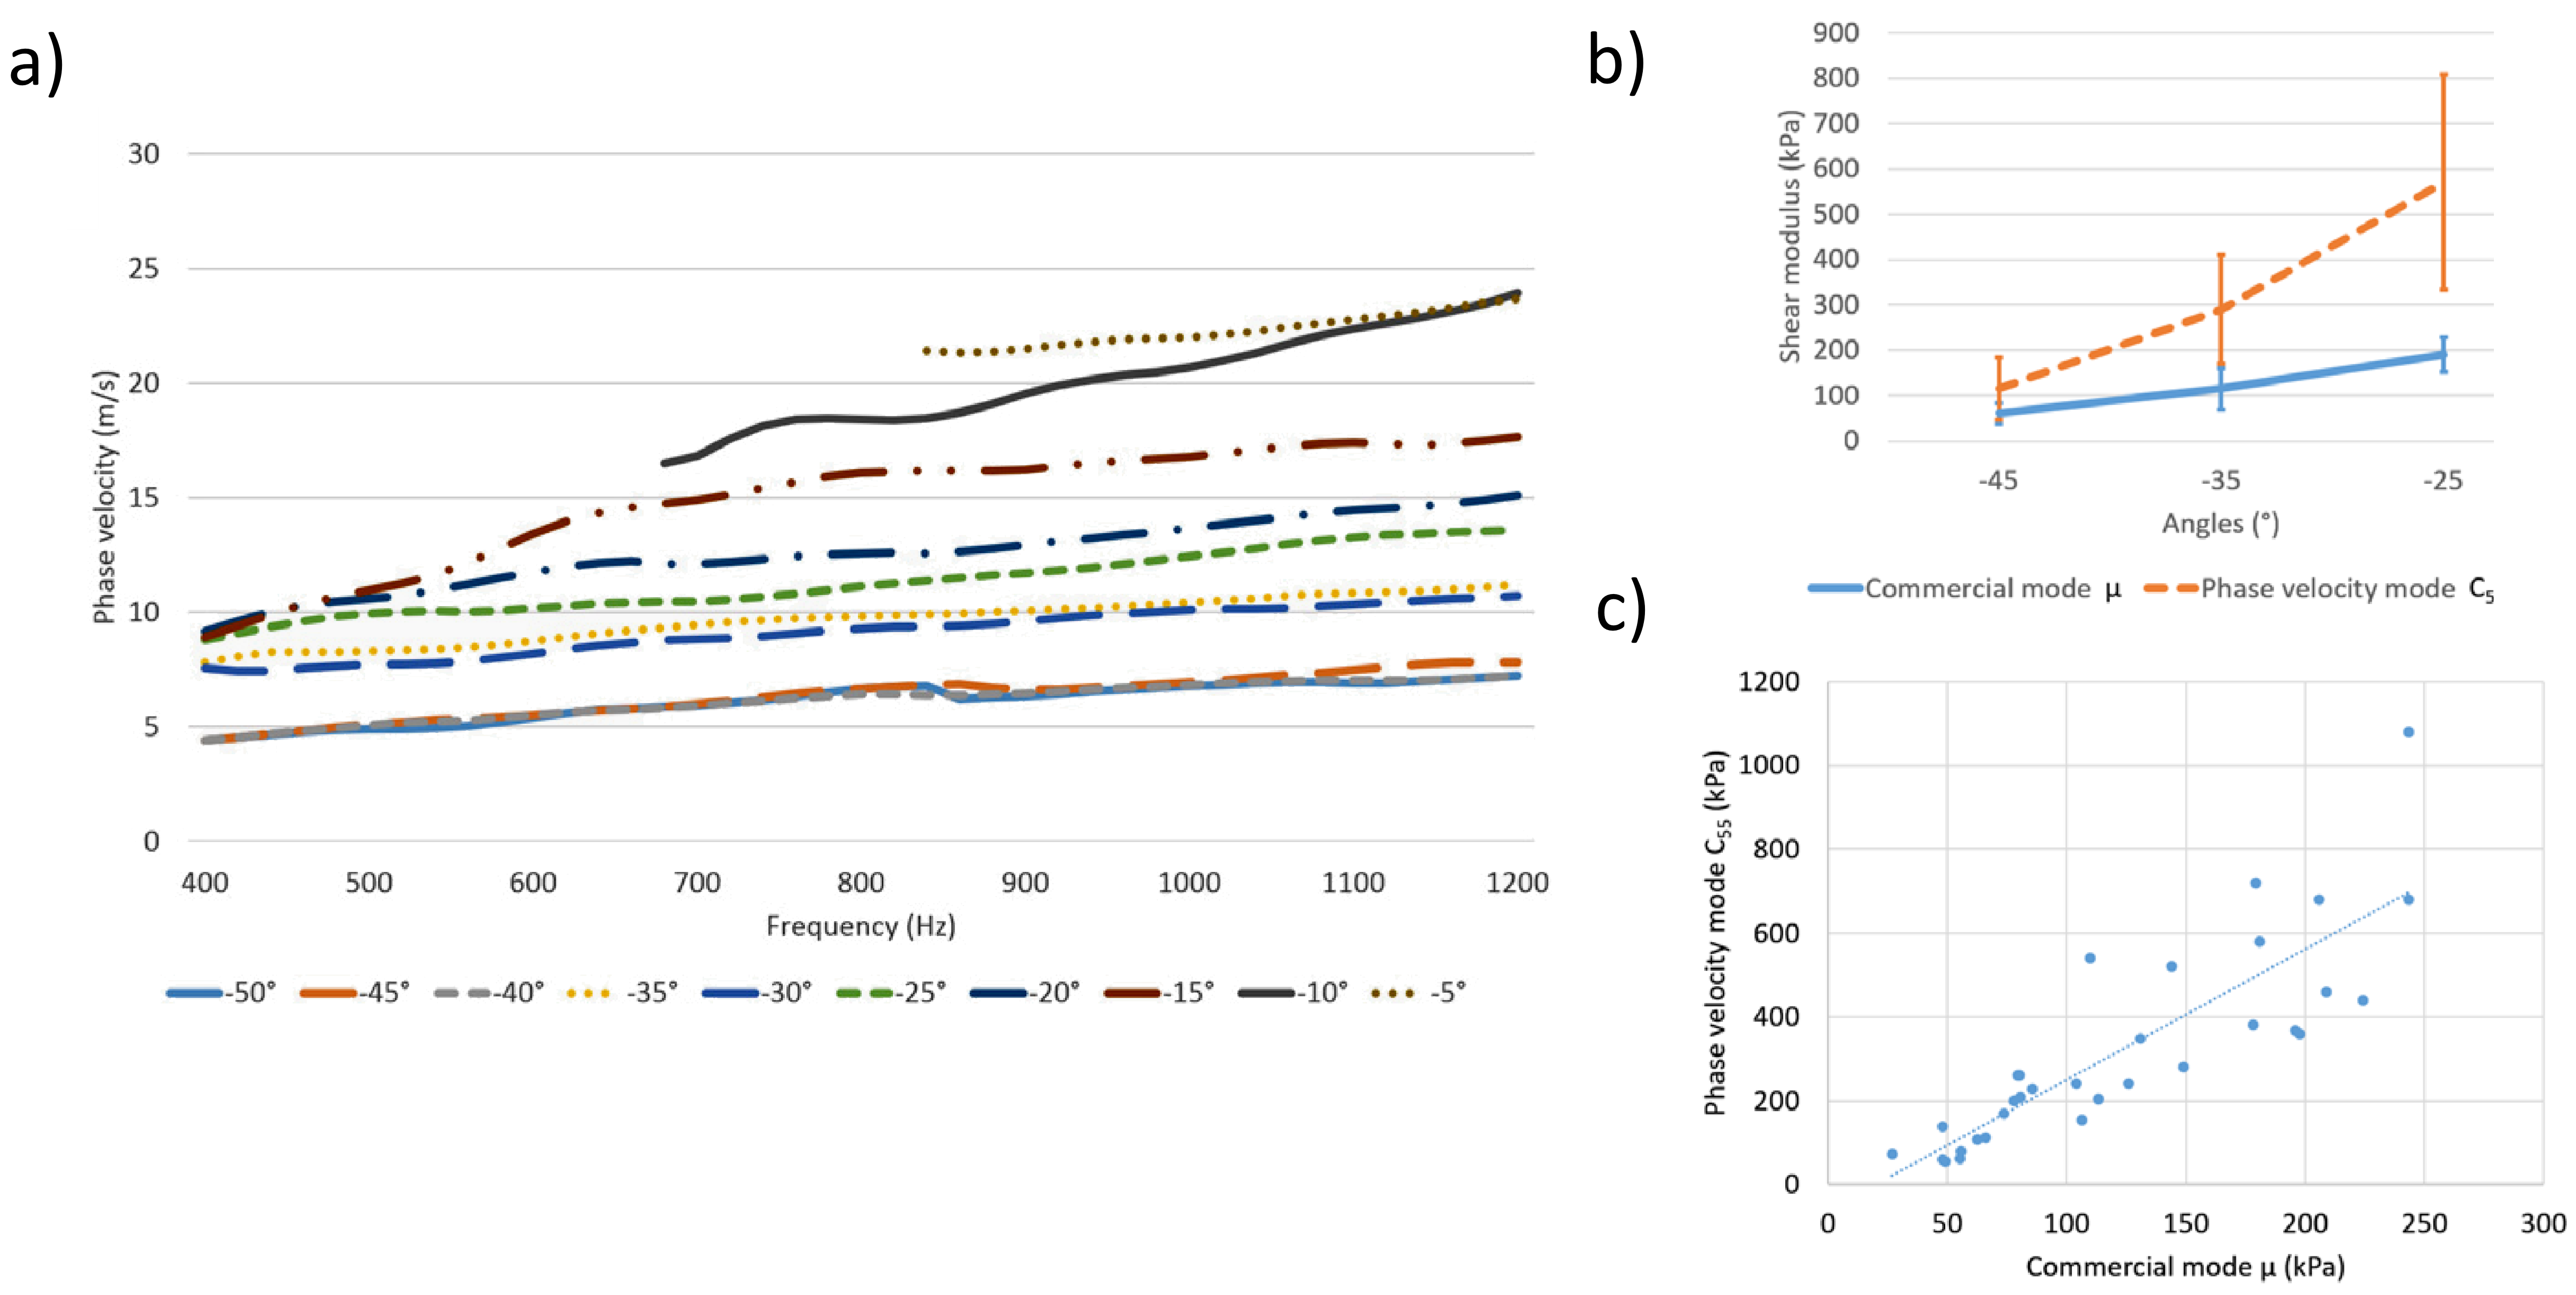
\includegraphics[width=\linewidth]{Figures/elastography/helfenstein_dispersion_angle.png}
	\caption{\textbf{(a)} Shear wave speed versus frequency for various ankle angles, negative angle denotes plantar flexion. Measured phase velocities for frequencies smaller than $c/h$ were removed, where $c$ is the measured shear wave speed and $h$ the mean tendon thickness (which was estimated from B-mode images). \textbf{(b)} Shear modulus assessed with SSI compared to the new method of \cite{brum_vivo_2014} for different plantar flexion ankle angles, \textbf{(c)} the linear relationship found between the two methods (correlation coefficient of $r=0.844$). Figure adapted from \citet{helfenstein-didier_vivo_2016}.}
	\label{fig:helfenstein_disperson_angle}
\end{figure}

\subsubsection{Dispersion analysis without shear wave guidance model}
\citeauthor{cortes_continuous_2015} did also perform a dispersion analysis, however they did not generate shear waves by acoustic radiation force, but used an external actuator in contact with the Achilles tendon via the skin \cite{cortes_continuous_2015}. Furthermore, no shear wave guidance model was used, and thus the viscoelastic properties were determined from the measured dispersion curves using a Voigt model (i.e. normal SWS method, in conflict with \cite{brum_vivo_2014, helfenstein-didier_vivo_2016}). Using the external actuator, a limited number of frequencies could be excited, from which the dispersion curves could be measured. The induced shear waves were imaged using ultrafast ultrasound, in the longitudinal direction (along the tendon). A strong viscoelastic effect was found in the tendon (ankle angle \SI{0}{\deg}), mean values of seven participants were reported to be $\mu_1 = 71.7 \pm 47.2$ \si{\kilo\pascal} and $\mu_2 = 64.6 \pm 13.3$ \si{\pascal\second}. 

	
	%Tendon rate dependency
	%====================================
	%"An important, often overlooked, physiological consideration is the viscous nature of tendons." \cite{seynnes_ultrasound-based_2014}
	%". In humans, a few studies, yet not all (49, 76), have confirmed the rate dependence of tendon mechanics in vivo (42, 74, 91) and in vitro (93); nonetheless, this property remains largely overlooked." \cite{seynnes_ultrasound-based_2014}
	%
	%
	%Nonlinear Force-elongation
	%====================================
	%"Tendon viscoelastic properties, and in particular the nonlinear force-elongation behavior of this tissue, is connected to another methodological challenge: the standardization of stiffness calculation. " \cite{seynnes_ultrasound-based_2014}
	%
	%
	%Tendon (+=muscle) moment arms + force estimation
	%====================================
	%"Unlike in vitro experiments or invasive procedures, the force exerted during in vivo tendon testing can only be estimated."
	%" Like all measurements performed in vivo, the estimation of moment arm length is bound to a number of assumptions that do not invalidate the use of these techniques. " \cite{seynnes_ultrasound-based_2014}
	




\subsection{Shear wave elastography in system identification}
Shear wave elastography may be applied neuromuscular system identification. In this context it may be able to measure the (visco)elastic properties of muscle and tendon tissue over its possible states, with as ultimate goal to determine the force in the MTU by relating measured displacements to stress. 
%The measurement of the (visco)elastic properties of muscle and/or tendon using elastography might be useful to estimate the force in the MTU, which can then be used to estimate the force in the muscle by using the material model to relate measured displacements to stress. 
Ultrafast ultrasound has enabled the development of two elastography methods, SSI and SWS. For the former, numerous studies have been conducted to measure the shear wave group velocity in a wide variety of tissues, including muscle and tendon. The latter is used only in a limited number of studies. This section first discusses the reliability of the various studies, followed by a proposed view on how these techniques can be used in system identification experiments. 

	%		- application of these shear wave speeds to system identification is not trivial. 
	%- study that estimates muscle force only demonstrated in very strict experimental conditions, hence questionable if applicable to other muscle groups. should first be demonstrated.
	%- limited frequency of shear modulus estimation, can be increased by using experimental settings. However, fast movement of muscles during identifying reflexes may distort estimation of shear wave velocity, is not demonstrated before. 


The estimation of muscle forces using SSI (\citet{bouillard_estimation_2011}) shows a linear relation between shear modulus and torque, albeit under very specific experimental conditions. During the very slow isometric contraction ramps SSI measurements at \SI{1}{\hertz} were performed, since this was the maximum sampling frequency of the used equipment. This is too slow for system identification experiments, however, it is known that SSI measurements can be performed at a much higher sampling frequency (by analysing the RF data after the experiment, see \autoref{sec:us_ssi} and \cite{bercoff_supersonic_2004}, under the assumption of sufficient memory). The slow contraction ramps show that it is possible to perform SSI while the muscle is moving slowly, but the contraction velocities encountered during reflexive activity are much higher. SSI measurements in comparable high velocity conditions have not been reported, and are probably impossible to conduct due to distortion of the shear wave on one hand, and the movement of speckles to track the shear wave propagation on the other hand (contribution to movement from both shear wave and contraction, complex to separate). Moreover, the method has not been tested for synergistic muscle groups, so the usability of the method when synergistic muscles are present remains unknown. 
%estimation of muscle force using SSI \cite{bouillard_estimation_2011,ates_muscle_2015} at 1 Hz only, not usable in sys ID. however, as demonstrated in SSI section, can be performed much faster if beamforming and analysis is not done in real time (which the aixplorer does). Hence, then the estimation of muscle force would be possible at X Hz. However, the muscle is moving a lot faster in sys id experiments than under the conditions of \cite{bouillard_estimation_2011,ates_muscle_2015}, resulting in distorted SSI measurement? Furthermore, this method has not yet been tested in synergistic muscle pairs.


%	- assessment of mechanical parameters can be done before sys id experiment, on muscle or tendon. 
Though the mechanical properties presumably cannot be assessed while performing identification trials, they can be measured prior and after the experiment in tendon and/or muscles. There is however quite some difference in the used elastography methods and reported material parameters across studies, and the results cannot be validated \textit{in vivo}. Given these published results, the applicability of SSI and SWS to quantitatively assess the muscle or tendon properties for system identification purposes remains questionable at the moment. 

	%- two methods (SSI SWS)
%- different reports per method
%- lots of different experimental conditions make results difficult to compare. variety in how results are reported make it difficult to compare. Furthermore differences in subject groups used per study, individual differences subjects make different methdos hard to compare
Especially regarding SWS, there is quite some difference in the exact implementation of the SWS technique and underlying model (with its introduced assumptions) to assess the viscoelastic properties of muscle and tendon. In addition, there is a lot variety in the experimental conditions used in each of these studies, making it hard to compare them. Furthermore, not every study obtains the same material parameters. For example, where \cite{brum_vivo_2014, helfenstein-didier_vivo_2016} reports that the viscosity parallel to the tendon fibres cannot be estimated from the dispersion curves, \cite{cortes_continuous_2015} reports values for both viscosity and elasticity. Moreover, it is hard to assess the influence of individual differences in the tested subjects based on the published literature, when mean values with standard deviation over all the participants are reported. This further hampers the comparison of the studies using SWS, and determining their reliability.

%- conversion of shear wave velocity to material parameters introduces a lot of assumptions. 
%- SSI relatively easy (Eby), but different 5G = E intead of 3 like in assumed elastic model. 
%- SWS conversion to stiffness not reported before.
%- this makes it perhaps more a qualitative method, based on the rheological model. measured shear wave speed and dispersion are only things that can be seen as qualitative measurements. 
In both SSI and SWS, the tissue is assumed to behave according to a certain rheological model, but validation of these models requires additional research. In case of SSI, a linear elastic isotropic model is used. With this material description, it is possible to estimate the shear elastic modulus from the shear wave group velocity via $\mu=\rho c_g^2$. Following this model, the Young's modulus is equal to $E = 3\, \mu$ (see \autoref{sec:us_ssi}). However, simultaneous material testing and SSI of brachialis swine muscles resulted in a linear fit where $E \approx 5\mu$ \cite{eby_validation_2013}. This shows that SSI can perform well in comparing the shear wave (group) velocity from subject to subject in a more qualitative manner, opposed to the general claim that SSI and SWS allow quantitative assessment of material properties. For SWS, a similar study like \cite{eby_validation_2013} to compare the viscoelastic muscle properties to mechanical tests is not reported. Furthermore, the estimation of muscle force from the shear moduli described by the Voigt model and measured muscle or tendon elongation has not been shown in literature before.
% the conversion of the Voigt model parameters shear elasticity and shear viscosity to mechanical parameters to estimate muscle forces has not been reported.


%		- assessment of muscle properties hard, studies have done it for passive properties of the muscle. Active properties are dependent on activation level, fibre length and velocity, making the estimation of the properties only possible for the force length curve, not force velocity. This limits its usability in sys id experiments.
%		- Alternatively, elastography can be done on tendon, since this is passive material, and thus is not dependent on activation level. However, the tendon is known to behave rate dependent, and has nonlinear force-elongation properties \cite{seynnes_ultrasound-based_2014}. For tendon the same limitation applies as for muscle, that the rate dependence cannot be easily determined. Furthermore, due to the limited thickness of tendons, shear waves reflect at boundaries for low frequencies, distorting the estimation of the viscoelastic properties. 
The reported shear wave velocities for the passive muscle over a range of joint angles show a good correspondence to the expected increase in stiffness \cite{gennisson_viscoelastic_2010}, based on the passive muscle tissue properties \cite{zajac_muscle_1989}. The active properties show a lot more variation (conflicting reports on dispersion), and are more difficult to identify, since they have to be measured for different joint angles and activation levels. Since elastography cannot be performed during eccentric or concentric contraction, the force-velocity characteristic cannot be obtained using elastography. This means that for a muscle, elastography could in theory only be used to separate the active and passive tissue contributions to stiffness in isometric and passive conditions. In dynamic conditions, as presented during system identification experiments, substantial MTU interaction is expected, which further limits the usability of the passive material parameters, because of the many possible combinations of joint angle, activation level and ratio between tendon and muscle length. Although the tendon has only passive properties (i.e. does not depent on activation signal), aforementioned reasons also limit the use of assessed tendon properties, of which the often neglected rate dependency cannot be assessed \cite{seynnes_ultrasound-based_2014}. 


It has been shown that the estimation of shear moduli using SSI varies with transducer pressure and ROI size in both muscle and tendon \cite{kot_elastic_2012}. Furthermore, the shear wave group velocity was found dependent on scanning depth and whether there was bone below the ROI \cite{ewertsen_evaluation_2016}. This calls on one hand for standardisation in performing elastography experiments, by e.g. using casts or mounts for the probe in which the pressure can be properly set and maintained, eliminating interobserver reproducibility issues (reported by e.g. \cite{aubry_biomechanical_2013}). On the other hand this shows the need for further research, e.g. to find the underlying physical principles for the variation dependent on surrounding tissue and depth. 

\tred[
It can be concluded that before elastography measurements can be of value in system identification, the current techniques require extensive validation. This can help in finding consensus on the appropriate models for various tissue types, or provide insight in the effects of using (simplified) models to aid the interpretation of the results. Currently, these effects are not sufficiently known, which hampers the relaxation of assumptions in neuromuscular system identification. 
]
%extensive research is needed to find the relation between the estimated shear wave velocity profiles and mechanical properties of muscle and tendon. However, under dynamic conditions, elastography may never be of use, despite technological progress. 


%\subsection{Sources of variation in elastography assessed properties}
%\citet{kot_elastic_2012}
%
%\citet{koo_factors_2015}
%
%\citet{ewertsen_evaluation_2016}
%- using elastography there is variation due to handling of probe, and different technical settings \cite{kot_elastic_2012}
%first e.g. probe mounts have to be developed, and the influence on the quantitative nature of the various  elastograpghy methods has to be further studied, before it is applicable to sys ID. Exact protocols have to be developed...
%
%- abundance of studies uses SSI to assess youngs modulus (e.g. [shinohara 2010, Arda 2011, maisetti 2012], ...see Brandenburg et al. 2014), however the quantitative nature of this measurement cannot be validated in vivo. The in vitro study of \cite{eby_validation_2013} validated this, but did not found the relation $E=3\mu$, but approximately $E=5\mu$. This difference indicates that it might be a more qualitative measurement, but since E is assumed to increase as function of the group velocity squared, the influence on the error in estimation might be limited... 
%
%- for elastography compound imaging can be used to increase image quality, but alternative beamforming methods (Garcia 2013, Montaldo 2009) /RF remapping (check Sumanaweera 2005) can also be used to improve image quality, without decreasing effective frame rate %\cite{cortes_continuous_2015}
%







%\newpage











% ===========================================================================
\section{Separating proprioceptive contribution -- imaging}
Besides elastography, ultrafast imaging can be used to track the elongation of muscle fibres, tendon and/or displacement of the myotendinous junction (MTJ). This is expected to be especially useful in understanding the contribution of the different proprioceptive afferents to observed joint movement. 

Ultrafast ultrasound has been used by a number of studies to image skeletal muscle, though the majority of studies use the technology for elastography. Currently, ultrafast imaging has not been used to study reflexes, or to acquire additional data for system identification of the neuromuscular system. Muscle fibre behaviour and MTU interactions during voluntary or electrically stimulated contrations have been studied using ultrafast ultrasound. The findings of these studies will first be presented. 
%In this section first an overview of the findings with ultrafast imaging of the MTU wil be presented. 
Hereafter, studies that used conventional ultrasound to identify the contribution of the components of the MTU (and thus the afferent activity) to reflexes and their findings will be shown. \tred[It will then be discussed in what way ultrafast imaging can help in understanding the origin of the afferent feedback, in what way this can help to fill the existing gap in knowledge and validation of current hypotheses, and finally how this can be useful when trying to relax assumptions in system identification studies. ]
% \tred[XXX not really relating to system identification, more to identifying stretch reflex]

%% LOCATIONS TO IMAGE
%Imaging can be done at three locations; \textbf{(1)} Over the muscle belly to obtain fibre length of one or more muscles with similar function (e.g. \cite{klint_afferent_2009, cronin_triceps_2015}) 
%\textbf{(2)} Muscle tendon junction, fibre and tendon length (e.g. \cite{klint_afferent_2009})
%\textbf{(3)} Tendon to obtain tendon elongation 


% ===========================================================================
\subsection{Ultrafast imaging of muscle and tendon}
\label{sec:ufus_muscle_tendon}
%Several studies demonstrated the use of ultrafast ultrasound imaging of muscle and tendon during movement, though the identification of reflexes mediated by afferent feedback using ultrafast ultrasound has not been demonstrated before. 

% DEFFIEUX VELOCITY PROFILE
\citet{deffieux_ultrafast_2006} were the first to use ultrafast ultrasound to image the contraction of muscle fibres in vivo upon electrical stimulation (\SI{30}{\volt} for \SI{400}{\micro\second}). The \textit{biceps brachii} was imaged at \SI{1500}{\hertz}, and using the cross correlation between two successive RF signal recordings the local particle velocity could be assessed, in axial direction (i.e. ultrasound beam transmit direction). This resulted in a particle velocity profile that corresponds to the lateral widening of muscle fibres, instead of their actual shortening. The spatial resolution in the axial direction is much higher than in the longitudinal direction (elaborated further in \autoref{sec:ufus_disc_sys_id}). With this method a maximum particle velocity (i.e. muscle fibre widening) of about \SI{0.7}{\centi\meter\per\second} was found. The muscle fascicle length per frame was not assessed, and due to the fusiform shape and limited size of the ultrasound probe, it is not possible to determine the absolute length of the fibres \cite{hodges_measurement_2003}. Consequently, only relative length changes can be assessed for the \textit{biceps brachii}. This group later performed a study similar to \cite{deffieux_ultrafast_2006}, and named the used tracking technique `echo mechanomyography' \cite{deffieux_assessment_2008}. However, after this last study, the technique has not been reported again. 


% HAURAIX MTU CONTRIBUTIONS DURING ISOKINETIC PLANTAR FLEXION
\citet{hauraix_shortening_2013} used ultrafast ultrasound to determine the contributions of the different components of the MTU during isokinetic plantar flexions. Imaging was performed at four locations (during four separate trials), over the muscle belly of the medial gastrocnemius and the lateral gastrocnemius, and the myotendinous junction of both these muscles. Six different isokinetic angular velocities (30, 90, 150, 210, 270, and \SI{330}{\deg\per\second}) were used to determine the contributions of MTU components, while ankle angle, velocity and torque were measured. Ultrasound imaging was performed at a maximum of 1000 frames per second. One location per trial was imaged, hence each condition was repeated four times to image all the locations once. A good repeatability was found for all the conditions, except for the initial \SI{10}{\deg} of motion, which was therefore omitted from the analysis. This allowed all the measurements to be combined, as depicted in \autoref{fig:hauraix_2013}. It was found that the contributions of tendon and muscle to plantar flexion are highly velocity and angle dependent, see \autoref{fig:hauraix_2013_contrib}. 


	% HAURAIX 2013
	\begin{figure}[!t]
		\centering
		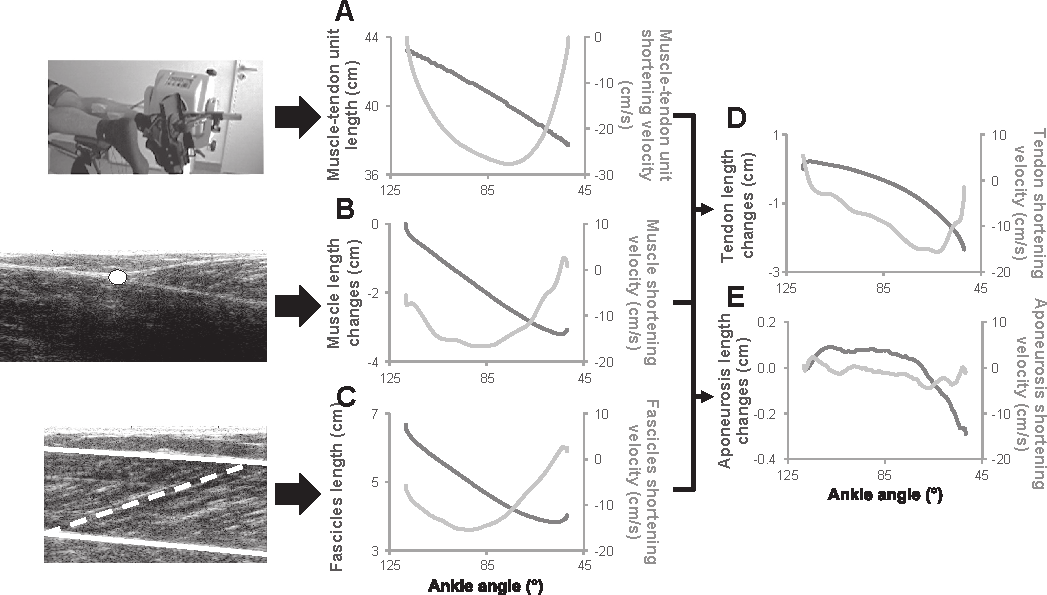
\includegraphics[width=\linewidth]{Figures/mtu_imaging/hauraix_2013_mtu_velocity.pdf}
		\caption{Overview of measured data by \citeauthor{hauraix_shortening_2013} for an isokinetic velocity of \SI{330}{\deg\per\second}. Since the data over the different trials for the different imaging locations showed good repeatability, the data could be combined. \textbf{(A)} From the ankle angle the total MTU length was estimated using as kinematic model. \textbf{(B)} From the ultrasound images the location of the myotendinous junction was tracked, from which the muscle length change was estimated. \textbf{(C)} From imaging over the muscle belly, the muscle fibre length was estimated, using the tracking algorithm of \citet{cronin_automatic_2011}. \textbf{(D)} From the difference in MTU length and muscle length, the tendon length change was determined. \textbf{(E)} Similarly, the aponeurosis length change was determined by the difference in muscle length and horizontal fibre length (i.e. horizontal component of line depicted in (C). Figure adapted from \citet{hauraix_shortening_2013}}
		\label{fig:hauraix_2013}
	\end{figure}
	
	% HAURAIX 2013
	\begin{figure}[t]
		\centering
		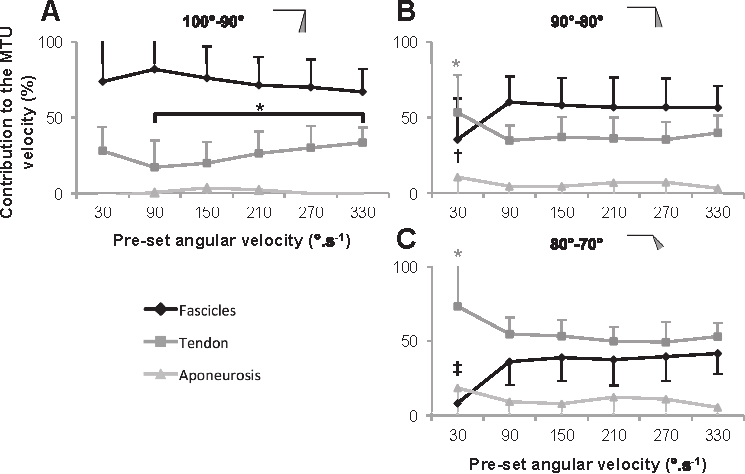
\includegraphics[width=.8\linewidth]{Figures/mtu_imaging/hauraix_2013_mtu_contrib.pdf}
		\caption{The relative contributions of tendon, fibres and aponeurosis for the different isokinetic velocity conditions, at three angle ranges. Significant differences with the fastest isokinetic condition are denoted by * ($P<0.05$), $\dag$ ($P<0.01$) and $\ddag$ ($P<0.001$). Figure adapted from \citet{hauraix_shortening_2013}}
		\label{fig:hauraix_2013_contrib}
	\end{figure}

% FARCY MTU CONTRIBUTIONS QUICK RELEASE GM
Similarly, \citet{farcy_interaction_2014} studied the contributions of the MTU components in quick releasing of the gastrocnemius medialis, from different levels of maximum voluntary contraction (30\% to 80\% MVC). Ultrafast ultrasound imaging at 2000 frames per second was performed with the probe location over the muscle belly, and over the myotendinous junction (again one location per trial). Good repeatability of the measurements (high intraclass correlation coefficients and low coefficients of variation) allowed averaging of the data, and combining the data of the two different imaging locations. It was found that for all MVC conditions, the tendon contributed significantly more ($P<0.01$) to lengthening of the MTU than muscle fibres and the aponeurosis. 
%This holds for all MVC conditions and the complete duration of the quick release trials. 
Furthermore, the relative contribution of the three components did not change with MVC level and the contribution remained constant over the complete trial duration (which was taken as a \SI{25}{\milli\second} window after releasing), except for the first \SI{5}{\milli\second}. 






% ===========================================================================
\subsection{Conventional imaging of muscle and tendon}
There is an abundance of studies using conventional ultrasound to image the muscle or tendon. For example, this has led to the understanding that MTU length is not necessarily representative for muscle fascicle length, and thus for MS Ia and II afferent activity, e.g. \cite{maas_is_2009, cronin_automatic_2011}. In addition, though the frame rate is limited, many insights relating to afferent feedback have been reported using this imaging technique. These will be discussed hereafter. 



\subsubsection{Afferent feedback during locomotion}
%expectation? Klint? Sinkjaer? GTO expected more than MS? Timing? Loram? 
%No studies using ultrafast ultrasound for imaging of tendon or muscle displacement. Studies using conventional B-mode ultrasound in abundance.
Ultrasound imaging has been used to assess the muscle fascia length during locomotion by e.g. \citet{klint_afferent_2009}. By lowering a hydraulically actuated platform during locomotion, it was found that there was a depression in soleus activity (EMG) at a latency of \SI{42}{\milli\second}, while the muscle fascicle started to differ from the normal walking condition (i.e. no platform drop) after \SI{54}{\milli\second}. This indicates that not MS but GTO feedback via the Ib afferent modulates late stance locomotion. These findings were in correspondence to an earlier study by \citet{grey_positive_2007}, in which plantar flexion perturbations (rapid unloading) during locomotion were applied directly at the ankle, while tendon force was measured using a buckle transducer. 


\subsubsection{Stretch reflex}
Tracking of muscle fascicles using conventional ultrasound has also led to new insights in the stretch reflex. \citet{cronin_triceps_2015} found a poor correlation between fascicle stretch (evoked by Achilles tendon tapping and dorsiflexion by ankle dynamometer) of the \textit{triceps surae} and the short latency reflex (SRL). The poor correlation between the the SLR size and magnitude of both muscle fascicle length and velocity, were in conflict with the earlier belief that the Ia and II afferent muscle spindle activity are the main contributors to characteristic SLR EMG response (e.g. \cite{schuurmans_monosynaptic_2009}). Instead, recorded mechanical vibrations in the limb induced by the tendon taps, were thought to be the main contributor to MS Ia activity. It was thought that the vibrations cause the muscle fibres to oscillate, and consequently result in oscillations in the muscle spindles, which are believed to be sensitive to oscillation amplitudes of at least \SI{5}{\micro\meter} (in cat muscles \cite{brown_relative_1967}). 

%The tendon taps evoked vibrations in the muscle, which were believed to induce oscillations in the muscle spindles. 
%Same for fascicle velocity, Ia and II afferents thus were found to not really contribute to stretch reflex. Magnitude of applied stretch was not correlated to magnitude observed stretch reflex. 
%\tred[MORE oscillation hypothesis... NO!]

%Due to availability ultrasound equipment, and possible interference us waves (?) ultrasound performed at one place. By purely imaging, US can result in tendon length, fibre length, or both. These measurements can be used to estimate the lengthening velocities. 
%However, at one location, only agonist muscles can be imaged, not both at the same time with limited equipment.  



% ===========================================================================
\subsection{Ultrafast imaging in system identification}
\label{sec:ufus_disc_sys_id}
%\textbf{assumptions to Relax}
%\begin{itemize}
%	\item Proportion of contribution of afferent and voluntary can be modelled. Model origin of EMG signal.
%	\item one MTU infinitely stiff tendon
%	\item sources of afferent feedback \tred
%\end{itemize}
%\textbf{intro discussion}

\tred[draft:] To gain a better understanding in how applied mechanical perturbations result in the observed motor behaviour, more data has to be gathered about muscle fibre and tendon behaviour during various experiments. Therefore, first the stretch reflex will be looked at, since it is \tred[thought] to be monosynaptic, and therefore easier to identify then motor behaviour involving many synapses (and voluntary, upper motor neuron... ). 

When looking at the stretch reflex, it is clear that ultrafast ultrasound can be used to determine the latency of muscle fascicle stretch with a higher temporal resolution. In addition to this, ultrafast imaging may also be of use to \textbf{(1)} validate the muscle spindle oscillation hypothesis (which \citeauthor{cronin_triceps_2015} could not test) \textbf{(2)} measure possible influence of the Ib afferent on the stretch reflex and \textbf{(3)} relate measured EMG activity during joint dynamic system identification experiments to the imaged movement of different elements of the MTU. 

%Methods to validate these hypotheses will be presented. 
%The proposed methods could also be used on the ultrasound data that can be acquired in joint dynamic system identification experiments. The use of these methods, and finally, in what way these can help in relaxing assumptions will be discussed at the end of this section.
%Then, these analysis techniques can also be used on the ultrasound data that is acquired in system identification experiments. 


% TABLE AND FIG with spatial resolutions. 
% Table generated by Excel2LaTeX from sheet 'Sheet1'
\newcolumntype{L}[1]{>{\raggedright\let\newline\\\arraybackslash\hspace{0pt}}m{#1}}
\newcolumntype{C}[1]{>{\centering\let\newline\\\arraybackslash\hspace{0pt}}m{#1}}

% Table generated by Excel2LaTeX from sheet 'Sheet1'
\begin{table}[t]
	\centering
	\caption{Properties of different transducer types, and the axial and longitudinal resolution.}
	\small
	\begin{tabular}{L{2cm}C{2.5cm}C{1.8cm}C{1.8cm}C{1.8cm}C{1.8cm}}
		\toprule
		Transducer      & {center frequency [MHz]} & {number of elements} & {max depth [mm]} & {axial res. [\si{\micro\meter}]} & {longitudinal res. [\si{\micro\meter}]} \\
		\midrule
		L12-5 50mm      & 7.813           & 256             & 77              & 19.7            & 195 \\
		L12-5 38mm      & 7.813           & 192             & 77              & 19.7            & 195 \\
		L38-22v 18mm    & 30              & 256             & 20              & 5.1             & 70 \\
		\bottomrule
	\end{tabular}%
	\label{tab:transducer_specs}%
\end{table}%

\begin{wrapfigure}{r}{0.35\textwidth}
	\centering
	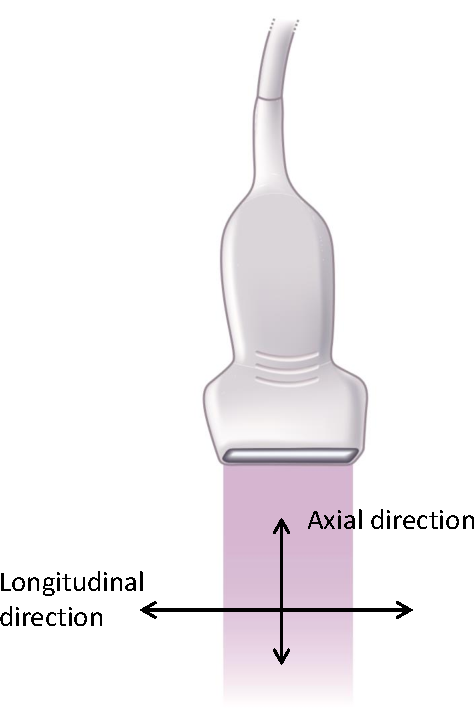
\includegraphics[width=0.9\linewidth]{Figures/Ultrasound/us_res_probe.pdf} 
	\caption{Overview of the important directions in 2D ultrasound imaging. The axial direction is the direction in which the beam is emitted, and the direction perpendicular to this in the imaging plane is referred to as the longitudinal direction. Figure edited from \citet{martin_basic_2011}.}
	\label{fig:usresprobe}
\end{wrapfigure} \leavevmode

%
%\begin{figure}
%	\centering
%	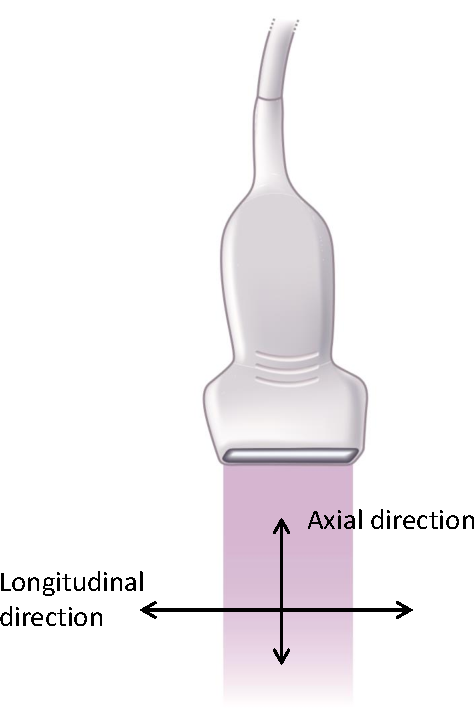
\includegraphics[width=0.3\linewidth]{Figures/Ultrasound/us_res_probe.pdf}
%	\caption{Figure edited from \citet{martin_basic_2011}.}
%	\label{fig:usresprobe}
%\end{figure}



\subsubsection{Spatial resolution ultrafast ultrasound}
The spatial resolution that can be achieved is largely dependent on the type of probe that is used. Furthermore, displacement analysis can be done using two techniques, that are fundamentally different. On one hand, beamformed images can be used, in which the movement of groups of pixels can be tracked. This method is used in most studies that track muscle fascicle behaviour under dynamic conditions, and can be applied to both conventional and ultrafast ultrasound (e.g. \cite{farris_ultratrack_2016, farcy_interaction_2014, hauraix_muscle_2017, af_klint_sudden_2009, cronin_triceps_2015, cronin_automatic_2011}). The spatial resolution in axial and longitudinal direction (see \autoref{fig:usresprobe}) that can be obtained with this method, is indeed dependent on the transducer (number of elements per unit length, used frequency acoustic wave) and the number of pixels in the image. 

\tred[draft:] On the other hand, the raw RF signals recorded from backscattered echoes can be used to detect displacements.  due to the high sampling rate of the RF data, spatial resolution in the axial direction is much higher than longitudinal (as depicted in \autoref{tab:transducer_specs}). sample rate for RF data only limited by the sample rate of the analog to digital converter in the equipment. This method was called `echo mechanomyography' (see \autoref{sec:ufus_muscle_tendon}) by \citet{deffieux_assessment_2008}. In mechanomyography, \tred[only] displacements in the axial (ultrasound beam) direction can be assessed, by performing 1D cross correlation on the recorded RF signals of successive backscatters. 
%\tred[In comparison with tracking of muscle fibres in beamformed images (e.g. \cite{farris_ultratrack_2016}), the global velocity profiles can be regarded less meaningful. ] \tred[not necessarily less meaningfull, just showing something else. one global, one local...]

% ULTRASOUND SPATIAL RESOLUTION
(about a tenth of the ultrasound wavelength, approx. \SI{150}{\micro\meter} for a probe with a centre frequency of \SI{8}{\mega\hertz}), due to the high sampling rate of the RF data. The spatial resolution in the longitudinal (i.e. probe aperture width) direction is much lower, due to the limited number of piezoelectric transducers per unit length in the ultrasound probe, and the fact that this 

%larger in axial then transverse (?) direction (see \autoref{fig:usresprobe}). 
%influence probe frequency, width, number of elements per unit length.



\subsubsection{1. Stretch reflex muscle spindle feedback}
% stretch reflex temporal resolution --> but other approaches possible
%MOVED TO INTRO: {
%When looking at the stretch reflex, it is clear that ultrafast ultrasound can be used to determine the latency of muscle fascicle stretch with a higher temporal resolution. In addition to this, ultrafast imaging may also be of use to \textbf{(1)} validate the muscle spindle oscillation hypothesis (which \citeauthor{cronin_triceps_2015} could not test) and \textbf{(2)} measure possible influence of the Ib afferent on the stretch reflex. }


\tred[PROBLEM, how to invoke oscillations. How to identify contributions of that 'external' oscillation to oscillation in MS?]

% muscle spindle osscilation hypothesis: displacement field spectroscopy
%\subsubsection{Muscle spindle oscillation hypothesis}
To validate the hypothesis that muscle spindle oscillations are the main contributor to the observed intensity of the stretch reflex, some of the analysis techniques employed in SSI and SWS may be of use. In SSI, shear waves can be tracked with millimeter resolution in a multiple centimeter wide image \cite{deffieux_shear_2009}. To improve this spatial resolution, as is required for SWS, multiple experiments are conducted, from which the velocity fields can be averaged. This results in a submillimeter resolution, which allows determining the phase difference of relatively high frequent shear waves ($100-800$\si{\hertz}) over a distance of about \SI{1}{\centi\meter} (see \autoref{sec:us_sws}). In both SSI and SWS, the RF data is beamformed to an image, and the shear wave is tracked by cross-correlating consecutive frames. 

A similar approach might be applicable to determine the oscillations of muscle spindles, by doing a frequency analysis on the displacement field of the muscle fibres. Evoking the stretch reflex with low variation between trials in one subject (i.e. high repeatability) may be an issue, since a high repeatability in motor response or SLR (M1) latency does not guarantee high repeatability in local muscle fibre deformation (as becomes clear from the fascicle length traces for one subject in Fig. 1 of \cite{cronin_triceps_2015}). 

On the other hand, this experiment does not need a large probe to induce and follow the shear wave, but a smaller probe with a higher frequency and more transducers per unit length can be used. This does impose a limit on the muscles that can be analysed, since a the ultrasound waves with higher frequency will attenuate more (see \autoref{tab:transducer_specs}), hence only superficial muscles can be analysed.  
% -- XXX \tred[(superficial muscle ???), YES higher frequency probe --> more attenuation, only superficial muscle]. 
Since muscle spindles are $4-7$\si{\milli\meter} in length \cite{smith_chapter_2007}, the ROI to image can be much smaller, allowing to image only a portion of a muscle fibre. It needs to be assessed how representative this local behaviour is for the global muscle movement, and to what extend it is possible to image a single fibre with high spatial resolution. If the spatial resolution in a single experiment with a smaller, high frequency probe is sufficient, then the questionable repeatability does not form an issue any more. 

Another method would be to analyse the raw RF data instead of the beamformed images. As discussed before, the spatial resolution in the axial direction is much higher due to high sample rate, and as a result \citeauthor{deffieux_assessment_2008} showed that it is possible to reach micrometer resolution to image muscle fibre widening and thinning during contractions \cite{deffieux_assessment_2008}. By performing 1D cross-correlation between consecutive backscatters (i.e. RF data frames) the displacement of the fibre boundaries in the imaging plane can be tracked. In the longitudinal direction the spatial resolution will not increase using this method, due to the dependency on the number of elements per unit length in the probe. With this method, depending on the probe orientation, the cross sectional area or the fibre thickness can be tracked. The analysis of the fibre thickness in this case will be influenced by both the pennation angle of the muscle fibres and the transducer orientation. It may not always be possible for a pennate muscle to orient the transducer in such a way that the CSA of the fibres are imaged. Deviations from the ideal imaging plane, may lead to \tred[under- or overestimation] of the fibre thickness per frame, and thus muscle spindle oscillation and hypothesised Ia and II afferent activity. 

%and given the presumption that muscle spindles are sensitive to length changes larger than about \SI{5}{\micro\meter} \cite{cronin_triceps_2015}
% (muscle spindle length $4-7$\si{\milli\meter} \cite{smith_chapter_2007}), \tred[therefore less wide ultrasound probe, i.e. more transducers per unit length increases lateral resolution REF.] Since muscle spindles are sensitive to length changes from \SI{5}{\micro\meter}. 
%In SWS shear wave has to be distinguised from steady tissue, where in this case, all movement that occurs is of interest, but the oscillations have an unknown frequency and amplitude, making it hard to separate them from possible noise (low SNR).
%--> problem, out of imaging plane movement, no effect on perturbation frequency?, but has effect on estimation of amplitude oscillation (as in \cite{seynnes_ultrasound-based_2014}, underestimation fibre length). 



\subsubsection{2. Stretch reflex Golgi tendon organ feedback}
% Ib afferent activity, MTU force hard to estimate
%\subsubsection{}
The Golgi tendon organ is completely overlooked in the discussion in \citet{cronin_triceps_2015}. 
Stated by Cronin: "Moreover, increasing preactivation torque was often associated with a larger SLR but smaller and/or slower fascicle stretch (Fig. 3)." Preactivation: muscle stiffer, hence elongation more by tendon, raise in MTU force, raise in Ib afferent activity? 
Since the force in the MTU is hard measure and estimates are hard to validate (noninvasively), and thus the GTO Ib afferent activity, perhaps an alternative method can be used to estimate the Ib afferent activity. % uitwerken: XXX

Imaging at MTJ, where GTOs are positioned, in transverse plane to find tendon cross sectional area (CSA) over time.  \citeauthor{obst_three-dimensional_2014} found an observable difference in the Achilles tendon CSA between rest and at 70\% (isometric) MVC using conventional ultrasound \cite{obst_three-dimensional_2014}. In this study, a 3D scan was made of the tendon, by moving the probe between frames, a method that cannot be used in dynamics conditions. 

Perhaps worth exploring if there exists a correlation between tendon thickness and Ib afferent (excitatory) activity. Given the fact that spatial and temporal resolution of ultrafast ultrasound is sufficient to observe the tendon deformation during various contraction conditions. 

% problem with tendon thickness
Tracking the tendon CSA during experiments as the stretch reflex does run into the issue that the tendon is moving, and thus not only the tendon thinning, but also the varying thickness of the tendon will influence the measurement ... VAGUE. This causes an error that cannot be easily discriminated from the thinning (CSA decrease/increase unkown...), tendon CSA over its complete length also unkown, and highly dependent on the state / operating point.

Alternatively, the complete tendon can be imaged (\tred[name correct plane... not `complete']), and using speckle tracking the elongation of the tendon can be tracked. Then per location, the tendon thickness can be assessed. Given the fact that the spatial resolution is very high in the direction of the beam when analysing the RF data, this perhaps can be done with sufficient accuracy. I.e. being able to distinguish the elongation/shortening of the tendon and the changes in thickness (in one plane).


\subsubsection{3. Relaxing assumptions using ultrasound imaging}
%Source of Ia and II afferent feedback. 
%
%Ib afferent? 

During system identification (continuous) trials, above described measurement techniques could be used as well. By imaging the muscle belly, the muscle fibre length over time can be tracked. This data can used as a measure for Ia and II afferent activity, but due to the unknown $\gamma$ activation, does not have to be directly related to the afferent activity. Tracking of tendon elongation, CSA or thinning, could result in a measure for Ib afferent activity, which is more directly related to the true afferent activity, due to the absence of a \tred[sensitivity set system] as present in the muscle spindles. However, the integration of the Ib afferent does involve multiple interneurons, making it harder to relate motor behaviour to estimated Ib afferent.

These with ultrafast ultrasound obtained signals, i.e. fibre elongation and tendon deformation, could be used as inputs to a model that predicts EMG activity for either the agonist or antagonistic muscles. 





\subsubsection{Assumptions introduced by ultrasound imaging}
% Introducing additional assumptions in conformation
It must be noted that while trying to relax some assumptions using ultrafast ultrasound, new assumptions are introduced. The current ultrafast ultrasound equipment can image a 2D plane, in which the muscle fascicle can be tracked. However, in pennate muscles, the fibers in the muscle will rotate upon active contraction, hence move out of the imaging plane \cite{finni_structural_2006}. This out of plane movement, i.e. 3D conformation of the muscle belly, also appears in tendon, and will lead to a systematic underestimation of length changes \cite{seynnes_ultrasound-based_2014}. Consequently, tracking muscle fascicle to estimate the Ia and II afferent activity can also be underestimated, possibly in a non proportional manner (though as of now the gamma activation and thus MS sensitivity remains elusive). Ultrafast ultrasound can be extended to 3D imaging, as demonstrated by \citeauthor{provost_3d_2014} by creating a 3D plane wave, and performing 3D beamforming, but this is computationaly and memory-wise very expensive \cite{provost_3d_2014}. In the future, this would allow imaging the 3D confirmation of the muscle fibers, and thus accurate estimation of muscle fibre conformation and elongation. 
%When considering the complete MTU this may not directly be of influence, but when tracking muscle fascicle to estimate the Ia and II afferent activity, this may be of importance to take into account.
%Ultrasound imaging, tracking fascicle length introduces new assumptions: fibres move out of imaging plane, but assumed fully in plane %\cite{see discussion!}
%		- Finni - Finni (2006): During a contraction, the fibers in a pennate muscle rotate and there is shear strain in the interface between the muscle fibers (Gans, 1982; Huijing, 1999). 
%		-> US imaging only 2D plane, so out of plane fibre rotation is not taken into account. 
%		-  "Disregarding the 3D conformation of tendon introduces a systematic underestimation of tendon length and thus an overestimation of length changes." \cite{seynnes_ultrasound-based_2014}.


% ===========================================================================

\section{\tred[replacement] - Ultrafast imaging in system identification}
The shown literature on usage of ultrafast ultrasound to image muscle behaviour and the use of conventional ultrasound in system identification/studying reflex modulation shows that there is a huge potential for the application of ultrafast imaging to system identification. 

Hereafter the possibilities of applying ultrafast imaging to system identification will be presented, accompanied with an idea of which assumptions may be relaxed using this additional measurement data.



\subsubsection{Separate MTU contributions}
Linear assumption, low amplitude perturbations cause equal strain in MTU. MTU interaction purely estimated with parameters. Results of \citet{hauraix_shortening_2013} for intial 10 degrees (not reproducible) underline that this linear assumption could require validation. imaging of the MTU can one one hand be used to validate this assumption. 


\subsubsection{Separating source of afferent feedback}
IN addition to relaxing or validating the assumptions regarding MTU interaction, imaging of the MTU can aid in finding the source of afferent feedback. 
- fiber elongation and velocity measure for MS activity (Ia an II afferent). However influenced by $\gamma$-motoneurons. 
- tendon elongation possible measure for GTO (Ib) activity. The elongation of the tendon is then assumed to be a measure for the force in the MTU. 

As described before, the spatial resolution is much higher in the axial direction than in the longitudinal direction. Herefore it may be interesting to look at the thinning or thickening of muscle fibres and tendon. 

Story of overlooking GTO by Cronin. image tendon/MTJ CSA. Probe orientation matters, since tendon movement has to be assessed, correct change in CSA at location. 

Similar to the studies of \citet{af_klint_sudden_2009} and \citet{grey_positive_2007} where the platform drop is kind of a catch trial to find the difference between normal walking efferent activity and the efferent activity when the muscle is rapidly unloaded, could be done in sys ID experiments. XX found change in efferent activity before fibre length changes found, indicating GTO feedback. These kind of perturbations with catch trials can also be incorporated in system identification experiments. This does require a high repeatability in task execution (not quaruanteed since this is not motor behaviour that is as 'normal' as walking), and it has to be assessed whether the response to the catch trials is statistically different from the 'normal' trials. This would also assume that the modulation of afferent feedback remains constant during the perturbation (i.e. depending on the fusimotor set hypothesis). A similar catch trial like the rapid unloading must be thought of for fiber stretching, to be able to separate the MS feedback from the GTO feedback. 





\subsubsection{Reducing parameters to estimate}
Time delays often hard to estimate during parameter fitting procedure. Some studies do tendon tapping experiments to estimate the associated delays, but unknown MTU interactions still play a role in the found delay. UFUS can be used to find time delays in with higher certainty. Various experimental conditions can be presented, sudden stretch, catch trials, imaged tendon/fibre elongation can be related to change in expected EMG response (in case of catch trials). Time of first deviation from expected EMG can be a measure for time delay of the different proprioceptors. This possibly does require the introduction of the assumption that the afferent time delay does not vary with experimental condition, as the sensitivity of the afferent feedback is modulated by e.g. the 'fusimotor set' hypothesis (MS) and presynaptic inhibition (GTO). Changes in magnitude afferent feedback response still assumed modulated according to 'fusimotor set' hypothesis. 



\subsubsection{Delumping muscle groups}
multiple probe setup. agonist antagonists. 
Still synergistic muscles lumped. 
moment arms required. 
Further discussed in \autoref{sec:change_model_structure}.



% ===========================================================================
\section{Implementation ultrasound measurement in current NMC models}
\label{sec:rem_incompatibility}
The currently published neuromuscular models almost all share the assumptions of lumping all muscles (see \autoref{sec:rem_lumping-muscle}). This lumped structure greatly helps in reducing the number of parameters in the model, but induces a large gap between the defined parameters and their physiological meaning. With ultrafast ultrasound, it is possible to acquire data that is closer to the physiology (i.e. proportional), and therefore not directly compatible with the current parametric neuromuscular models. To use the acquired data to fit a model, either a substantial change in the model structure has to be made, or the experimental conditions have to be adapted. The specific model changes or exact experiment design is beyond the scope of this literature survey, however, some thoughts will be shared.

%When adding the UUS technology to the system identification experiments, this asks for a change in the experiment design and/or the model design. elongation of muscle or tendon measurements cannot be plugged in as input to the currently used model structures (agonist and antagonist lumped). Therefore, or the experiment has to be designed differently, or the model has to be adapted.



\subsection{Change in experiment design}
At the present time, ultrafast ultrasound equipment is very costly. For this reason, it will be assumed that there is only one ultrafast ultrasound device available in a lab. With a single ultrafast ultrasound device, only one side of a limb can be imaged, either the flexor or the extensor. Consequently, it is not trivial to identify the complete neuromuscular system. As a simplification, only one group of muscles could be identified, by avoiding activation of the antagonistic muscle group. This would mean that the joint has to be disturbed at a sufficient distance from the neutral position, to ensure that only the agonist can contribute to the rejection of the disturbance. To validate that the antagonist is not active during the experiment, EMG measurements can be used, as demonstrated in e.g. \cite{kearney_identification_1997, mirbagheri_intrinsic_2000}. The antagonistic MTUs do indeed still have a passive contribution to the movement, which still has to be identified. 

Alternatively, experiments similar to those of \citeauthor{de_gooijer-van_de_groep_estimation_2016} can be conducted \cite{de_gooijer-van_de_groep_estimation_2016}. In these experiments, a sudden strain is applied (participant asked to not interfere), and only reflexive activity in combination with passive properties are expected. These kind of transient experiments do not allow for the classical system identification (perturb system over wide band of frequencies), but could provide a lot of insight on the contribution of MS and GTO feedback, and subsequent force generation. The nonlinear model of \cite{de_gooijer-van_de_groep_estimation_2016} could relatively easy be expanded with an afferent feedback model, and could be useful to explain the observed movement based on the with ultrasound measured tendon or muscle elongation. 
%, apply strain, no voluntary activity, and try to fit reflex activity to activation of single muscle group (flexor or extensor group). Transient experiments under condition, no real sys ID, but could provide more insight in the contribution of GTO and MS
%Experimental conditions in which antagonistic muscle is not active (e.g. \cite{kearney_identification_1997, mirbagheri_intrinsic_2000}). Could be validated by EMG measurement. E.g. only positive torque, so that only agonist muscle is activated. Think of experimetal conditions such that the current model can be used to identify the properties of the agonist muscle, and tendon ... to identify the joint dynamics under those conditions. Real identification experiment over wide band of frequencies. No need to change the model structure (e.g. models as \cite{schouten_nmclab_2008, mugge_rigorous_2010}


\begin{figure}[t]
	\centering
	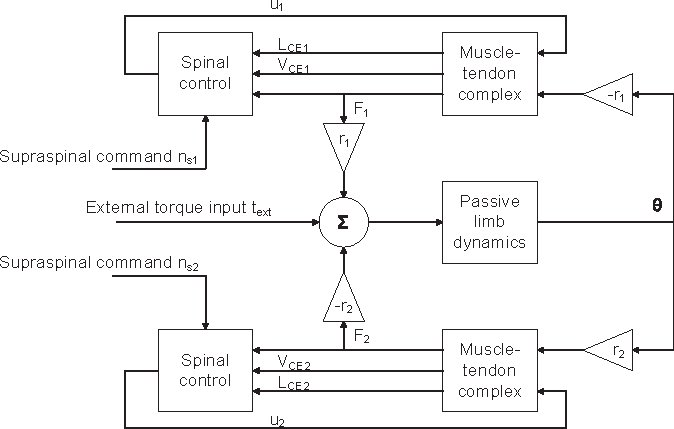
\includegraphics[width=.8\linewidth]{Figures/elastography/mugge_antagonistic.pdf}
	\caption{Antagonistic muscle model used in the simulation study of \citeauthor{mugge_modeling_2012}. The spinal control consists of MS and GTO feedback, and takes an additional supraspinal command as input. The force in the MTU is multiplied by a moment arm to obtain the joint torque. Figure adapted from \citet{mugge_modeling_2012}.}
	\label{fig:mugge_antagonistic}
\end{figure}


\subsection{Change in model structure}
\label{sec:change_model_structure}
Without a change in experiment design, the model structure has to be made compatible with the additional ultrasound measurement data. One possibility is the introduction of an antagonistic muscle model, like used in \cite{de_gooijer-van_de_groep_estimation_2016}. However, this study did not perform a complete system identification and did not attempt to identify the source of reflexive feedback as mentioned before. Neuromuscular models that include modelling of afferent proprioceptive feedback and antagonistic muscles cannot be found in the context of system identification, but are used in simulation studies, e.g. \cite{munts_fixed_2011, mugge_modeling_2012}. 

The model of \citeauthor{mugge_modeling_2012} (see \autoref{fig:mugge_antagonistic}) is nonlinear and consists of about 50 parameters \cite{mugge_modeling_2012}. It includes the nonlinear properties of the proprioceptors and MTUs (adopted from \cite{winters_analysis_1985, stroeve_neuromuscular_1998}). By contrast, the (linear) model of \citeauthor{schouten_nmclab_2008} consists of 18 parameters \cite{schouten_nmclab_2008}. The difference in linear versus nonlinear modelling makes the comparison unfair, since the linear model is in fact a linearisation of a nonlinear model. However, when considering a linear antagonistic neuromuscular model, this would require (at least) double the number of parameters to describe the MTUs and proprioceptors. In addition, moment arms are required to estimate the net joint torque, introducing at least two additional parameters that are not present in a lumped model. 

In the ideal case, not all of these additional parameters have to be estimated in the parameter fitting procedure. For example, the (average) moment arms could be determined by imaging techniques (MRI, ultrasound \cite{fath_direct_2010}) or estimated based on anthropometric data \cite{ramsay_muscle_2009}. When the relation between shear wave propagation and stiffness or even muscle force is more clearly established, elastography measurements could be used to estimate the tissue (visco)elastic parameters, further relieving the parameter estimation procedure. 

Under the assumption that only one ultrafast ultrasound system is available (costly equipment), only one group of muscles (with the same function) can be imaged during a identification experiment, either the flexors or extensors. Consequently, the sources of afferent feedback can only be estimated for one muscle group. Hence, the antagonistic MTU group remains kind of a black box, in which the MTU interaction cannot be separated. 

The first study that uses ultrafast ultrasound in system identification might have to change the experimental conditions together with the neuromuscular model. 


%In many studies, the muscle tendon unit interaction is omitted, or other methods to estimate the muscle and tendon elongation are used. EXAMPLES, studies that estimate using ankle angle… Not the way to go. The total elongation of the MTU can still be used, and the additional information of US can be used to quantify the individual contribution of lengthening, since one elongation of the (series) system is known. 

%To use this length information, the agonist and antagonist muscles should be modelled separately. But separating these muscle groups faces some difficulties, since the length information of only the agonist MTU is available from the measurement. The antagonistic MTU elongation can still only be estimated as a whole, not individual contributions. 
%Lengthening information of specific muscle can better explain some of the reflexes, but only at for one muscle / muscle group per function. Therefore, the most useful modelling structure will be analysed. 

%A study by \citep{mugge_modeling_2012, munts_fixed_2011} did use an antagonistic muscle model \tred[(INCLUDE MODEL SCHEME)], in which proprioception was included. This was however a (forward) simulation study, and no identification based on measured subject data. These two domains have to be linked, and perhaps UUS can be the bridge. \tred[haha].  

%Mugge et al. used an agonist-antagonistic muscle model to simulate movement patterns (relating to CRPS). This model structure was derived from (Winters \& Stark 1989) and (Stroeve 1998), and consists of an antagonistic muscle pair, both modelled by a Hill model. Describe equations. 

%Using US, there is however the problem that (depending on the equipment available) only one group of muscles (flexor or extensor) can be imaged. So when using two Hill models, the contributions of the other MTU are unknown. This can lead to wrong estimation of MTU elongation, and can lead to problems in identifying the reflexive contributions to movement (further discussed in section afferent feedback)
%Similarly, the intrinsic contributions also become more complicated, since e.g. the intertial contribution has to be split in minimal three components (MTU1, MTU2, limb etc) (further discussed in section intrinsic feedback).


%\subsubsection{Muscle-tedon unit modelling}
%Tendon properties can be assessed with SSI or SWS. 
%relating measurements to muscle force and subsequently joint torque. 
%Several studies not modelled anything, others based on Hill type muscle model. An alternative is the Huxley model, based on crossbridge attachment. 
%
%Hill, Huxley, no model?
%
%Discuss Hill, CE PE SE element. Parameters in model. 
%If antagonistic model is used, one side can be modelled as MTU, in which individual contributions M and T are known. 
%Other side however faces problem, since these separate contributions remain unknown. Here the estimation method employed by Mugge and Schouten perhaps is better. 
%
%
%Alternative, no model 
%Estimate the viscoelastic parameters of tendon (SSI elastography, Supersonic shear wave imaging).
%Measure elongation of tendon. 
%x and xdot of tendon times stiffness viscosity results in force. 
%Tendon properties known to be nonlinear, Finni 2006: “While the tendon force–length curve is non-linear, the Young’s modulus is typically derived from a linear portion of the stress–strain curve (Butler et al., 1978), with an approximate value of 1.2 or 1.5GPa (Zajac, 1989, Alexander, 2002).” 
%Test in multiple ankle positions. ???

